

% this file is called up by thesis.tex
% content in this file will be fed into the main document

%: ----------------------- introduction file header -----------------------
%\begin{savequote}[50mm]
%Personally, I think it does help, that it makes a beneficial difference, but the scientific literature on the subject is very messy.
%\qauthor{Jeanne Petrek}
%“And upon the top of the pillars was lily work: so was the work of the pillars finished.”
%
% Bible quotes
%\end{savequote}


\chapter{Monodrom\'ia de la ecuaci\'on hipergeom\'etrica}
\label{cha:State of the Art}

% the code below specifies where the figures are stored
%\ifpdf
 %   \graphicspath{{2_state_of_the_art/figures/PNG/}{2_state_of_the_art/figures/PDF/}{2_state_of_the_art/figures/}}
%\else
 %   \graphicspath{{2_state_of_the_art/figures/EPS/}{2_state_of_the_art/figures/}}
%\fi


%-------------------------------------------------------------------------

%\cite{turing1950computing}

En este cap\'itulo presentamos conceptos b\'asicos de la teor\'ia de ecuaciones diferenciales as\'i como definiciones y teoremas que son \'utiles para calcular la monodrom\'ia de la ecuaci\'on hipergeom\'etrica, enunciamos los teoremas sin demostraci\'on. Para las demostraciones podemos dirigirnos a \cite{gausspainleve}. \\

 En el caso m\'as general podemos considerar un sistema de ecuaciones diferenciales ordinarias de primer orden.

\begin{equation} \label{sistema ecuaciones diferenciales}
\frac{du_{j}}{dz} = f_{i}(z,u) \ \ \  (j=1,..,r)
\end{equation}

Con la variable independiente $z$ y el vector de inc\'ognitas $u=(u_{1},u_{2},..,u_{r})$, donde el vector $f=(f_{1},..,f_{r})$ es holomorfo en un dominio $D \subset \mathbb{C} \times \mathbb{C}^{r}$

\begin{thm} Para cada $(a,b) \in D $ hay una soluci\'on \'unica $u$ de \ref{sistema ecuaciones diferenciales} holomorfa en una variedad de $a$, tal que
\begin{equation} \label{u(a)=b}
 u(a)=b
\end{equation}
\end{thm}

\begin{thm} Si el sistema \ref{sistema ecuaciones diferenciales} y el valor inicial \ref{u(a)=b} depende de manera holomorfa de un sistema de par\'ametros $s=(s_{1},..,s_{r})$, entonces la soluci\'on es holomorfa en $x$ y en $s$
\end{thm}

El motivo de definir un sistema de este tipo es que todo sistema de ecuaciones diferenciales ordinarias de cualquier orden, se puede reducir a un sistema del tipo \ref{sistema ecuaciones diferenciales}.


\section{Ecuaciones lineales }

Consideremos la siguiente ecuaci\'on diferencial ordinaria;

\begin{equation}
\label{eqn:sistema_ecuaciones_ordinarias}
\frac{d^{r}u}{dz^{r}} + a_{1}(z) \frac{d^{r-1}u}{dz^{r-1}} + \cdots + a_{r}(z)u=0
\end{equation}

Donde las $a_{j}'s$ son holomorfas en un dominio $D \subset \mathbb{C}$, introducimos nuevas variables;

$$u_{0}=u \ \ \, u_{i} = \frac{d^{i}u}{dz^{i}} \ \ \ (i=1,..,r-1)$$

La ecuaci\'on \ref{eqn:sistema_ecuaciones_ordinarias} se puede reescribir de la forma :

\begin{equation}
\frac{du_{i}}{dz} = \sum_{j=0}^{r-1} a_{i}^{j}(z)u_{j} \ \ \ (i=0,...,r-1)
\end{equation}


\begin{thm}Para cada punto $a \in D$ y cualesquiera complejos $b_{0},..,b_{r-1}$ hay una \'unica soluci\'on holomorfa de \ref{eqn:sistema_ecuaciones_ordinarias} tal que

$$\frac{d^{i}u}{dz^{i}}(a) = b_{i} \ \ \ \ \ i=0,..,r-1$$

Dicha soluci\'on tiene una continuaci\'on anal\'itica a lo largo de cualquier curva en $D$.
\end{thm}

Si los coeficientes de la ecuaci\'on \ref{eqn:sistema_ecuaciones_ordinarias} son holomorfos en $\lbrace z \mid 0 < |z-a|< \epsilon  \rbrace $ para alg\'un $\epsilon > 0 $ y al menos una es meromorfa y no holomorfa en $\lbrace z \mid |z-a| < \epsilon \rbrace$, entonces el punto $a$ es un punto singular de \ref{eqn:sistema_ecuaciones_ordinarias}. \\

\begin{defn} Un punto singular $a$ de \ref{eqn:sistema_ecuaciones_ordinarias} es regular si

$$(z-a)^{k}a_{k}(z), \ \ \ \ (k=1,..,r)$$

Son holomorfas en $a$.
\end{defn}

\section{Comportamiento alrededor de puntos singulares regulares}

Consideremos $z=0$ un punto singular regular de la ecuaci\'on  \ref{eqn:sistema_ecuaciones_ordinarias} (en el caso de la ecuaci\'on hipergeom\'etrica $z=0$ es un punto singular regular). Como en \ref{sec:sol_ec_hip} introducimos el operador;

$$D= z\frac{d}{dz} $$

Este operador se relaciona con $\frac{d}{dz}$ de la siguiente manera,

\begin{equation}  \label{relacion-operadores-com-alr-pun-sing}  \ z^{k}\frac{d^{k}}{dz^{k}}= D(D-1) \cdots (D-k+1) \end{equation}

Para $k \geq 1 $ se tiene

$$ z^{r} \lbrace \frac{d^{r}}{dz^{r}} + a_{1}(z) \frac{d^{r-1}}{dz^{r-1}} + \cdots a_{r}(z) \rbrace \
= \sum_{k=0}^{r} z^{r-k}a_{r-k}(z)D(D-1) \cdots (D-k+1) \ $$
$$=D^{r} + \lbrace za_{1}(z) - \frac{(r-1)(r)}{2} \rbrace D^{r-1} + \cdots $$

Donde $a_{0}=1$.
La ecuaci\'on \ref{eqn:sistema_ecuaciones_ordinarias} se puede reescribir en la forma

$$ Lu=0 $$

Donde $L$ es un operador de la forma;

$$ L= \sum_{i=0}^{r} b_{i}(z) D^{r-i}$$

Donde $b_{0}(z) = 1$, y $b_{1}(z),..,b_{r}(z) $ estan dados por series convergentes. Escribimos;

\begin{equation}
  b_{i}(z)=\sum_{j=0}^{\infty} b_{ij}z^{j}, \ \  0 \leq i \leq r
\end{equation}

En particular, $b_{00}= 1, b_{0j}=0, \ \ \ (j \geq 1)$, escribiendo ;

$$ u= z^{s} \sum_{k=0}^{\infty} c_{k} z^{k}, \ \ c_{o}=1$$

Calculamos $Lz$:

$$Lz = \sum_{i=0}^{r} \sum_{j=0}^{\infty} b_{ij} z^{j} D^{r-i} \sum_{k=0}^{\infty} c_{k} z ^{s+k}$$
$$= \sum_{k=0}^{\infty} \sum_{j=0}^{\infty} \sum_{i=0}^{r} b_{ij} (s+k)^{r-i}c_{k}z^{s+k+j}$$
$$= z^{s} \sum_{n=0}^{\infty} \lbrace \sum_{k=0}^{n} \sum_{i=0}^{r}  b_{i,n-k}(s+k)^{r-i}c_{k} \rbrace z^{n} $$

Y teniendo en cuenta $Dz^{\alpha} = \alpha z^{\alpha}$, escribimos;

$$f(s) = \sum_{i=0}^{r} b_{i,0}s^{r-i} = \sum_{i=0}^{r} b_{i}(0) s^{r-i}$$

\begin{defn} La ecuaci\'on algebraica

 \begin{equation} \label{eqn:ecncarac} f(s)=0 \end{equation}

Se llama la ecuaci\'on caracter\'istica en el punto singular regular $z=0$. Las ra\'ices de \ref{eqn:ecncarac}  son llamados los exponentes caracter\'isticos.
\end{defn}

\section{ Ecuaciones Fuchsianas }

\begin{lem} Una ecuaci\'on diferencial
$$ \lbrace D^{r} + b_{1}(z)D^{r-1} + \cdots + b_{r}(z)  \rbrace u =0$$

Es regular singular en $z=0$ si y solo si $b_{j}, (1 \leq j \leq r)$ son holomorfas en $z=0$
\end{lem}

La ecuaci\'on \ref{eqn:sistema_ecuaciones_ordinarias} con coeficientes racionales es $Fuchsiana$ si cada punto singular en ${\mathbb{C}}$ es regular, y si despu\'es de un cambio de variable $z$ en $t=\frac{1}{z}$, la ecuaci\'on transformada tiene un punto singular regular en $t=0$. Los exponentes de $t=0$ son llamados los exponentes de \ref{eqn:sistema_ecuaciones_ordinarias} en el infinito.

\begin{prop}[Una caracterizaci\'on de las ecuaciones $Fuchsianas$ ]
La ecuaci\'on \ref{eqn:sistema_ecuaciones_ordinarias} es $Fuchsiana$ con singularidades regulares en $z_{1},...,z_{m},z_{m+1} = \infty $ si y solo si los coeficientes tienen la siguiente forma:

$$ a_{k}(z) = \frac{p_{k}(z)}{\prod^{m}_{i=1}  (z-z_{i})^{k}}, \ \ \ \ (k=1,..,r)$$

Donde cada $p_{k}(z)$ es un polinomio de grado a lo m\'as $k(m-1)$.
\end{prop}

\begin{defn} Un esquema de $Riemann$ es una tabla donde se representan los puntos singulares $z_{1},..,z_{m+1}$ y los exponentes en $s_{i}^{1},..,s_{i}^{r}$ en $z_{i}$, el esquema de $Riemann$ de \ref{eqn:sistema_ecuaciones_ordinarias} se expresa como



\[ \left( \begin{array}{ccc}
z_{1} & ... & z_{m+1} \\
s_{1}^{1} & ... & s_{m+1}^{1} \\
... & ... & ... \\
s_{1}^{r} & ... & s_{m+1}^{r} \end{array} \right)\]

\end{defn}

\section{Esquema de Riemann de la ecuaci\'on hipergeom\'etrica}

Para nuestra ecuaci\'on hipergeom\'etrica

\begin{equation}
\label{ecuacion_hipergeometrica}
 (1-z )z \frac{d^{2}u}{dz^{2}} + \lbrace  c -(a+b+1)z \rbrace \frac{du}{dz} -abu =0
\end{equation}

Deseamos hallar el esquema de Riemann  correspondiente, esto nos sirve para hallar la monodrom\'ia mas adelante por medio de las identidades de $Gauss-Kummer$ (\cite{gausspainleve}).

Los puntos singulares de nuestra ecuaci\'on son $1,0,\infty$, y esto lo podemos ver transformando la ecuaci\'on \ref{ecuacion_hipergeometrica} a la forma est\'andar;

$$ \frac{d^{2}u}{dz} + \frac{\lbrace c-(a+b+1)z \rbrace}{z(z-1)}\frac{du}{dz} - \frac{ab}{z(z-1)}u=0$$

Y obtenemos $a_{1}(z) = \frac{c- (a+b+1)z}{z(z-1)}$ y $a_{2}(z)=\frac{-ab}{z(z-1)}$, podemos ver que los puntos singulares son $0,1$ e $\infty$ (mostramos despu\'es que $\infty$ tambi\'en es un punto singular pero consideremos por ahora que esto es cierto). Estos puntos tambi\'en son regulares como podemos verificar;

Para $z=0$
$$za_{1}(z) = z (\frac{c-(a+b+1)z}{z(1-z)})= \frac{c-(a+b+1)z}{1-z}$$

Y

$$z^{2}a_{2}(z)=z^{2} (\frac{-ab}{z(1-z)})= \frac{-abz}{1-z}$$

Y ambas son holomorfas en $z=0$, an\'alogamente verificamos que $z=1$ es un punto singular regular (El caso $z= \infty $ se deja al final). Tenemos entonces 3 puntos singulares regulares para la ecuaci\'on \ref{ecuacion_hipergeometrica}, lo que deseamos ahora es hallar los exponentes en cada punto.\\

Para $z=0$ recordemos que los exponentes son las ra\'ices de la ecuaci\'on \ref{eqn:ecncarac}, la cual esta dada en este caso por
$$f(s) = \sum_{i=0}^{2} b_{i}(0) s^{r-i} $$

Y en este caso $b_{1}(z) = za_{1}(z) -1$ y $ b_{2}(z)= z^{2}a_{2}(z)$, es decir $b_{1}(z) = \frac{c-(a+b+1)z}{1-z} -1$ y $b_{2}(z) = \frac{-ab}{1-z}$ y por tanto;

$$f(s)= s^{2} +b_{1}(0)s + b_{2}(0) = s^{2} + (c-1)s +0 $$

Cuyas ra\'ices son 0 y $c-1$. Para encontrar los exponentes en $z=1$ hacemos un proceso similar y escribimos;

$$D_{1} = (z-1)\frac{d}{dz}$$

Y se cumple la misma relaci\'on de antes entre $D_{1}$ y $\frac{d}{dz}$, luego;

$$(z-1) \lbrace \frac{d^{r}}{dz^{r}} + a_{1}(z)\frac{d^{r-1}}{dz^{r-1}}+ \cdots + a_{r}(z) \rbrace = D_{1}^{r} + \lbrace (z-1)a_{1}(z) - \frac{(r-1)(r)}{2} \rbrace D_{1}^{r-1} + \cdots $$

Si llamamos $f_{1}$ a la ecuaci\'on caracter\'istica de \ref{eqn:sistema_ecuaciones_ordinarias} en $z=1$, tenemos en este caso $b_{1}(z)= (z-1)a_{1}(z) -1$ y $ b_{2}(z) = (z-1)^{2}a_{2}(z)$ entonces;

$$ f_{1}(s) = s^{2} + b_{1}s + b_{2}(1)= s^{2} + \lbrace c-(a+b+1) +1 \rbrace s = s^{2} - (c-a-b)s $$

Cuyas ra\'ices son $0$ y $c-a-b$. Basta hallar los exponentes para $z= \infty$, hacemos una transformaci\'on $t=\frac{1}{z}$ y definimos $\theta \frac{t}{dt}$ y notamos que $D=- \theta$, obtenemos entonces;

$$z^{r} \lbrace \frac{d^{r}}{dz^{r}} + a_{1}(z) \frac{d^{r-1}}{dz^{r-1}} + \cdots +a_{r}(z) \rbrace = \sum_{k=0}^{\infty} t^{-(r-k)}a_{r-k} (\frac{1}{t})(-1)^{k} \theta (\theta +1) \cdots (\theta + k-1)$$

En nuestro caso, para $r=2$ la ecuaci\'on es

$$\theta^{2} + (1-t^{-1}a_{1}(\frac{1}{t}))\theta + t^{-2}a_{2}(\frac{1}{t}) $$

Donde $-t^{-1}a_{1}(\frac{1}{t}) = \frac{a+b+1-ct}{t-1}$ y $t^{-2}a_{2}(\frac{1}{t})= \frac{-ab}{t-1}$ de aqui vemos dado que ambas son holomorfas en $0$ que $z= \infty$ es un punto regular singular. Entonces si $f_{\infty}$ denota la ecuaci\'on caracter\'istica de \ref{ecuacion_hipergeometrica} con el cambio de variable en $t=0$, tenemos;

$$ f_{\infty}(s) = s^{2} + (-a-b)s +ab$$

Cuyas ra\'ices son $a$ y $b$, por tanto los exponentes en $z=\infty $ de \ref{ecuacion_hipergeometrica}  son $a$ y $b$. Concluimos con el esquema de $Riemann$ de la ecuaci\'on hipergeom\'etrica  esta dado por

\[ \left( \begin{array}{ccc}
0 & 1 & \infty \\
0 & 0 & a \\
1-c &c-a-b & b  \end{array} \right)\].

\section{Monodrom\'ia}

Si consideramos de nuevo la ecuaci\'on \ref{eqn:sistema_ecuaciones_ordinarias}, es posible asociarle una clase de conjugaci\'on en $GL(2,\mathbb{C})$ a la cual llamamos la monodrom\'ia de \ref{eqn:sistema_ecuaciones_ordinarias}. Consideremos el grupo fundamental $\Pi_{1} (D,b)$ donde $D$ es una vecindad en la cual los coeficientes de \ref{eqn:sistema_ecuaciones_ordinarias} son holomorfas y $b \in D$.\\

Sea $U$ una vecindad simplemente conexa de $b \in D $ y sea $\mathfrak{F}= (u_{1},..,u_{n})$ un sistema fundamental de soluciones en $U$. Si $\alpha \in \Pi_{1}(D,b)$ sea $\gamma$ un representante y $\gamma_{*} \mathfrak(F)$ la continuaci\'on anal\'itica de $\mathfrak{F} $ a lo largo de $\gamma$. El teorema de monodrom\'ia para la continuaci\'on anal\'itica (\cite{gausspainleve}) implica que $\gamma_{*} \mathfrak{F}$ depende en la clase de homotopia $\alpha$, podemos escribir entonces $\alpha_{*} \mathfrak{F}$ en lugar de $\gamma_{*} \mathfrak{F}$. Ya que \ref{eqn:sistema_ecuaciones_ordinarias} es lineal, $\alpha_{*} \mathfrak{F}$ es tambi\'en un sistema fundamental de soluciones de \ref{eqn:sistema_ecuaciones_ordinarias} en $U$ y hay una \'unica matriz invertible $M(\alpha; \mathfrak{F}) \in GL(n,\mathbb{C})$ tal que

\begin{equation} \label{relacionmatrizsisfun}
\alpha_{*} \mathfrak{F} = \mathfrak{F} M(\alpha;\mathfrak{F})
\end{equation}

Ya que $e_{*} \mathfrak{F} = \mathfrak{F}$ y $(\alpha \beta)_{*} \mathfrak{F} = \alpha_{*} (\beta_{*} \mathfrak) $ para $\alpha ,\beta \in \Pi_{1} (D,b) $ tenemos

$$M(e,\mathfrak{F}) = I , M(\alpha \beta ;\mathfrak{F}) = M(\alpha ;\mathfrak{F})M(\beta ;\mathfrak{F}) $$

Esto implica que el mapeo

$$\rho_{\mathfrak{F}}: \Pi_{1} (D,b) \rightarrow GL(n,\mathbb{C}), \alpha \mapsto M(\alpha ; \mathfrak{F}) $$

Es un homomorfismo. Llamamos a $\rho_{\mathfrak{F}}$ la representaci\'on de monodrom\'ia y a $\rho_{\mathfrak{F}}(\Pi_{1} (D,b)) \subset GL(n, \mathbb{C})$ el grupo de monodrom\'ia de \ref{eqn:sistema_ecuaciones_ordinarias} respecto al sistema fundamental de soluciones $\mathfrak{F}$. Si $\mathfrak{G}$ es otro sistema de soluciones en otro punto $a$ y denotamos tambi\'en por $\mathfrak{G}$ la continuaci\'on anal\'itica de este a lo largo de una curva que une $a$ y $b$, existe una matriz $C \in GL(n,\mathbb{C})$ tal que $\mathfrak{G} = \mathfrak{F} C$ y tenemos

$$\mathfrak{G} M(\alpha ; \mathfrak{G})=\alpha_{*} \mathfrak{G} = (\alpha_{*} \mathfrak{F}) C  = \mathfrak{F} M(\alpha ; \mathfrak{F}) C = \mathfrak{G} C^{-1 } M(\alpha ; \mathfrak{F}) C $$

Es decir

$$M(\alpha ; \mathfrak{F}) = C^{-1} M(\alpha ; \mathfrak{F} )C$$

En otras palabras

\begin{equation} \label{4.1.3relacion}
\rho_{\mathfrak{G}}(\alpha)=C^{-1} \rho_{\mathfrak{F}}(\alpha) C, para \ \alpha \in \Pi_{1} (D,b)
\end{equation}

la representaci\'on de monodrom\'ia no solo depende de la ecuaci\'on diferencial \ref{eqn:sistema_ecuaciones_ordinarias}, depende de igual manera del sistema fundamental de soluciones. Notemos que de cualquier manera que \ref{4.1.3relacion} implica que cada par de representaciones de monodrom\'ia de \ref{eqn:sistema_ecuaciones_ordinarias} son conjugadas, tal que la clase de conjugaci\'on de la representaci\'on de monodrom\'ia se determina \'unicamente por la ecuaci\'on diferencial \ref{eqn:sistema_ecuaciones_ordinarias}. A esta clase de conjugaci\'on la llamamos $La \ Monodromia$ de \ref{eqn:sistema_ecuaciones_ordinarias}. entonces el grupo de monodrom\'ia $\rho_{\mathfrak{F}} (\Pi_{1} (D,b))$ de \ref{eqn:sistema_ecuaciones_ordinarias} respecto de cualquier $\mathfrak{F} $ pertenece a la misma clase de conjugaci\'on, que tambie\'n llamamos $La \ Monodromia$ de \ref{eqn:sistema_ecuaciones_ordinarias}.


Cuando \ref{eqn:sistema_ecuaciones_ordinarias} es una ecuaci\'on diferencial fuchsiana en la esfera de Riemann con puntos singulares regulares en $p_{1},..,p_{m},p_{m+1} = \infty$, se toma $D= \mathbb{C} \backslash \lbrace p_{1},..,p_{m} \rbrace$. Para cada $j=1,..,m$, sea $U_{j}$ un disco abierto en $D \cup \lbrace p_{j}\rbrace$ centrado en $p_{j}$, y sea $\textit{l} _{j}$ un lazo en $U_{j} \backslash \lbrace p_{j} \rbrace$ con punto base $q_{j} \in U_{j} \backslash \lbrace p_{j} \rbrace$ que encierra $p_{j} $ una vez en sentido antihorario, y sea $\mathfrak{F}_{j}$ un sistema fundamental de soluciones de \ref{eqn:sistema_ecuaciones_ordinarias}  en una vecindad simplemente conexa de $b$ y $\gamma_{j}, (j=1,..,m)$  arcos con punto inicial $b$ y punto final $q_{j}$. Las matrices de conexi\'on $C_{j} \in  GL(n, \mathbb{C}), \ (j=1,..,m)$ se definen por

\begin{equation}\label{eqn:matcon1}
  \gamma_{j_{*}} \mathfrak{F} = \mathfrak{F}_{j} C_{j}
\end{equation}

\begin{prob}{Problema de matrices de conexi\'on} Para una ecuaci\'on diferencial lineal dada, sean $\mathfrak{F}, \mathfrak{F}_{j}$ y $C_{j}$ como antes. Encontrar una expresi\'on explicita de las $C_{j}$.

Las matrices de circuito $M_{j}$ alrededor de $p_{j}$ se pueden definir por

\begin{equation}\label{eqn:matcon2}
 \textit{l} _{j_{*}} \mathfrak{F}_{j} = \mathfrak{F}_{j} M_{j}
\end{equation}

\end{prob}

Ya que los generadores del grupo de monodrom\'ia respecto a $\mathfrak{F}$ estan dados por

$$C_{j}^{-1} M_{j} C_{j} ,$$

Notamos que el problema de monodrom\'ia es parte del problema de conexi\'on.



\begin{figure}[h] \label{lazos3}
  \centering
  % Requires \usepackage{graphicx}
  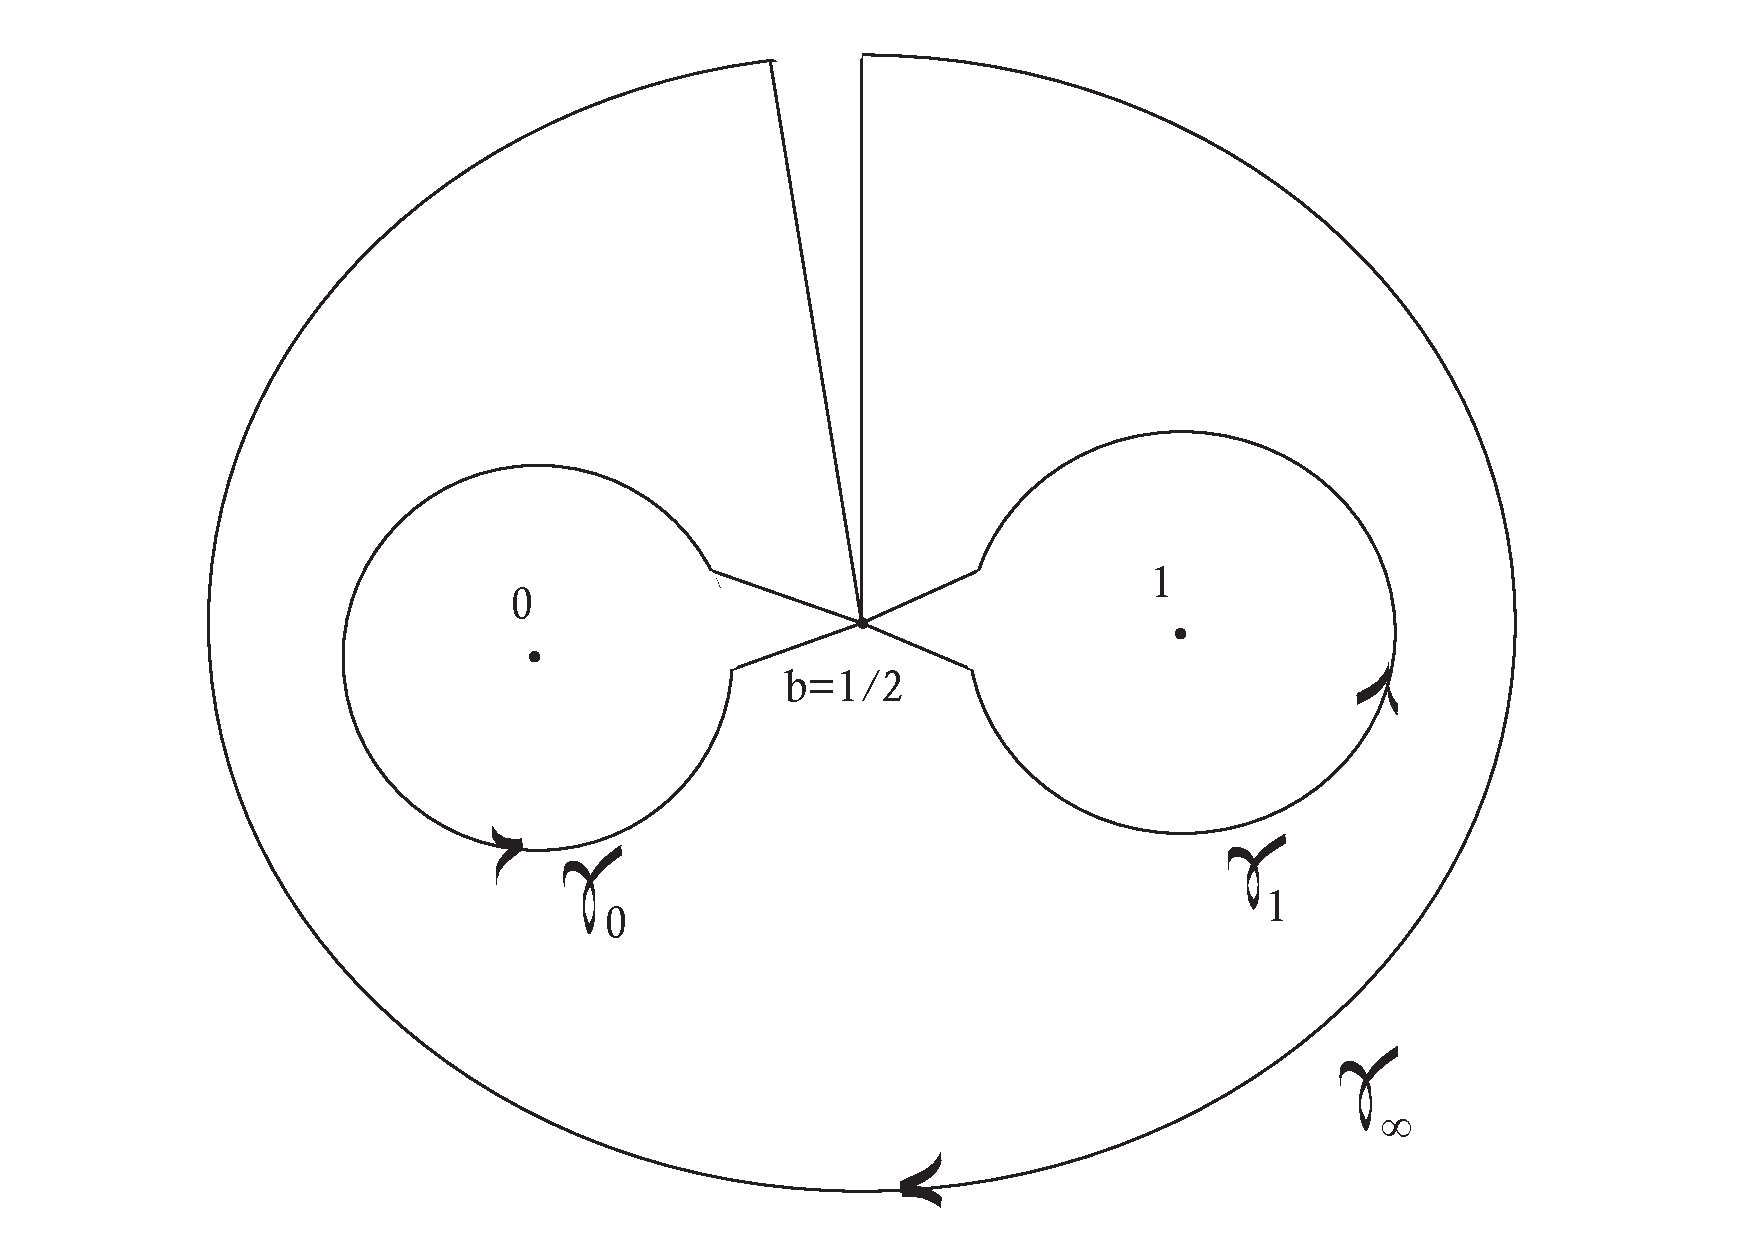
\includegraphics[width=10cm]{lazos3.pdf}
  \caption{Lazos anclados en $b=\frac{1}{2}$} \label{lazos3}
\end{figure}


El problema de hallar la monodrom\'ia respectiva a una ecuaci\'on diferencial es un problema complicado, afortunadamente existen m\'etodos que nos permiten hallar (en ciertos casos) la monodrom\'ia de la ecuaci\'on hipergeom\'etrica y tambi\'en el grupo de monodrom\'ia para soluciones particulares. En los siguientes cap\'itulos hallamos la monodrom\'ia de la ecuaci\'on hipergeom\'etrica y uno de los grupos de monodom\'ia respecto de las soluciones dadas en \ref{sec:sol_ec_hip}.


\section{Monodrom\'ia de la ecuaci\'on hipergeom\'etrica}

En esta secci\'on encontramos la monodrom\'ia de la ecuaci\'on hipergeom\'etrica a traves de su esquema de Riemann por medio de propiedades locales y la relaci\'on de Fuchs, utilizando fuertemente que la ecuaci\'on hipergeom\'etrica resulta ser irreducible.

Sea $G=\pi_{1} (D,b) $ y $\gamma_{j} \in G, (j=0,1,\infty )$, lazos en $b$. Sea $\rho: G \rightarrow GL(2,\mathbb{C}) $ una representaci\'on de monodrom\'ia del esquema de Riemann

\[ \left( \begin{array}{ccc}
0 & 1 & \infty \\
\rho_{1} & \sigma_{1} & \tau_{1} \\
\rho_{2} &\sigma_{2} & \tau_{2}  \end{array} \right)\]


Dado que 
\begin{equation}
\rho (\gamma_{1} \cdot \gamma_{0}) = \rho(\gamma_{\infty})^{-1}
\end{equation}

 ya que 
 \begin{equation}
 \gamma_{\infty}^{-1}=\gamma_{1} \gamma_{0}  y \gamma_{0}\gamma_{1}        
 \end{equation}
 
 
 es conjugado a $\gamma_{1} \gamma_{0}$, tenemos;

\begin{eqnarray} %equation
 \label{eqnarray:ecuacion1} \lbrace \varepsilon (\rho_{1}), \varepsilon (\rho_{2}) \rbrace \ conjunto \ de \ eigenvalores \ de \ \rho (\gamma_{0}) \\
 \lbrace \varepsilon (\sigma_{1}), \varepsilon (\sigma_{2}) \rbrace \  conjunto \ de \ eigenvalores \ de \ \rho (\sigma_{1}) \\
\lbrace \varepsilon(-\tau_{1}), \varepsilon (-\tau_{2}) \rbrace \  conjunto \ de \ eigenvalores \ de \ \rho (\sigma_{0} \sigma_{1})
\end{eqnarray}

Donde $\varepsilon (\cdot) = exp(2 \pi i \cdot)$. La clase de conjugaci\'on de $\rho$, es decir la monodrom\'ia de $RE(\rho,\sigma,\tau)$ esta casi determinada por los eigenvalores, y esta completamente determinada si la monodrom\'ia es irreducible.

\begin{defn}La ecuaci\'on de Riemann $RE(\rho,\sigma,\tau)$ se dice irreducible s\'i la monodrom\'ia es irreducible
\end{defn}

\begin{thm} \label{riemann-irreducible}

La ecuaci\'on de Riemann es irreducible si y solo si

$$\rho_{i} + \sigma_{j} + \tau_{k} \notin \mathbb{Z}, (i,j,k=1,2)  $$
Bajo esta condici\'on la representaci\'on $\rho $ se expresa hasta conjugaci\'on por las siguientes matrices:

$$ \rho (\gamma_{0}) \leftrightarrow  \begin{pmatrix}
 \varepsilon(\rho_{1})& 1\\
 0& \varepsilon(\rho_{2})
 \end{pmatrix}  ,\ \ \
\rho (\gamma_{1}) \leftrightarrow \begin{pmatrix}
 \varepsilon(\sigma_{1})& 0\\
 b& \varepsilon(\sigma_{2})
 \end{pmatrix}
$$

 Y el n\'umero $b$ esta dado por $b= \varepsilon(-\tau_{1}) + \varepsilon(-\tau_{2}) - \varepsilon(\rho_{1} + \sigma_{1}) - \varepsilon(\rho_{2} + \sigma_{2})$, y $\varepsilon(\cdot) =exp(2 \pi i \cdot)$. Todas las representaciones  obtenidas al intercambiar $\rho_{1},\rho_{2}$ y/o $\sigma_{1},\sigma_{2}$ son mutuamente conjugadas.

\end{thm}

En nuestro caso tenemos el esquema de Riemann;

\[ \left( \begin{array}{ccc}
0 & 1 & \infty \\
0 & 0 & a \\
1-c &c-a-b & b  \end{array} \right)\]

Y verificamos si satisface las condiciones del teorema, tenemos los siguientes casos:


\begin{enumerate}
\item 0+0+ a = a
\item 0 + c-a-b + b = c-a
\item 0 + c-a-b + a = c-b
\item 1-c + 0 + a= 1-c +a
\item 1-c + 0 + b=1-c+b
\item 1-c + c-a-b + b = 1-a
\item 0 + 0 + b = b
\item 1-c + c- a- b + a = 1-b
\end{enumerate}


 Queremos calcular $a,c-a,c-b,1-c+a,1-c+b,1-a,b,1-b$, y estamos considerando que los exponentes $ 1-c,c-a-b,a-b$ son imaginarios puros, por lo que basta probar que ninguno de los anteriores estan en $\mathbb{Z}$.

No es dif\'icil verificar que $b = \frac{1-i(\theta_{0} + \theta_{1} +\theta_{2})}{2} \notin \mathbb{R}$. Para $a$ tenemos;

$$a= \frac{1-i(\theta_{0} + \theta_{1} - \theta_{2})}{2}$$

Y podemos ver que $a \notin \mathbb{R}$ o $ a = \frac{1}{2}$  de cualquier modo $a \notin \mathbb{Z}$. Para $c-a$ se tiene;

$$c-a = \frac{1 + i (-\theta_{0} + \theta_{1} - \theta_{2})}{2}$$

Por lo que de nuevo $c-a \notin \mathbb{R}$ o $c-a = \frac{1}{2}$, y de cualquier modo $c-a \notin \mathbb{Z}$. Para $c-b$ se tiene;

$$c-b =\frac{1+i(\theta_{2} + \theta_{1} - \theta_{0})}{2} $$

Entonces $c-b \notin \mathbb{R}$ o $c-b =\frac{1}{2}$ y en cualquier caso $c-b \notin \mathbb{Z}$. Para $1-c+a$ notamos que $1-c+a= - (c-a-1 )$ y $c-a-1 = -\frac{1}{2}$ o $c-a-1 \notin \mathbb{R}$. En los casos restantes un proceso an\'alogo nos enseña que ninguno de los n\'umeros considerados esta en $\mathbb{Z}$.

Invocamos el teorema \ref{riemann-irreducible} al esquema de Riemann que hallamos para nuestra ecuaci\'on, y obtenemos que las matrices que generan la monodromia de la ecuaci\'on hipergeom\'etrica con exponentes imaginarios puros son:

$$ \rho (\gamma_{0}) \leftrightarrow  \begin{pmatrix}
 1& 1\\
 0& e^{2 \pi i (1-c)}
 \end{pmatrix}  ,\ \ \
\rho (\gamma_{1}) \leftrightarrow \begin{pmatrix}
 1& 0\\
 b& e^{2 \pi i (c-a-b)}
 \end{pmatrix}
$$

Con $b = e^{-2 \pi i a} + e^{-2 \pi i b} -1 -e^{2 \pi i (1-a-b)}$, y la monodrom\'ia de la ecuaci\'on hipergeom\'etrica es generada por $\rho (\gamma_{0}), \rho (\gamma_{1})$ en $GL(2, \mathbb{C})$.


\section{Grupo de monodrom\'ia con las soluciones dadas por la serie hipergeom\'etrica}

 En este cap\'itulo pretendemos dar a conocer el grupo de monodrom\'ia con el par de sistemas fundamentales de soluciones hallados en \ref{sec:sol_ec_hip}, utilizando las identidades de $Gauss-Kummer$. El enfoque principal en este cap\'itulo es exponer las herramientas necesarias para ese prop\'osito y los resultados principales que llevan a una expresi\'on del grupo de monodrom\'ia con los sistemas fundamentales de soluciones dadas. Los teoremas y resultados de este cap\'itulo pueden encontrarse en \cite{gausspainleve} as\'i como sus demostraciones, y se remite al lector a dicha bibliograf\'ia para un desarrollo m\'as profundo de lo expresado aqu\'i. \\


 Queremos resolver el problema de conexi\'on utilizando las identidades de $Gauss-Kummer$ y encontrar generadores para el grupo de monodrom\'ia de la ecuaci\'on diferencial hipergeom\'etrica con las soluciones dadas en \ref{sec:sol_ec_hip}. Los sitemas fundamentales de soluciones son $(f_{0}(x;0),f_{0}(x;1-c))$ y $(f_{1}(x;0),f_{1}(x;c-a-b))$ , queremos encontrar una relaci\'on entre estos sistemas.

 \begin{thm} Si ninguno de los exponentes $c$ o $c-a-b$ es un entero entonces

 $$ \label{relacion_sistemas_soluciones} (f_{0}(x;0),f_{0}(x;1-c))=(f_{1}(x;0),f_{1}(x;c-a-b))P$$

 Donde $P$ es la matriz definida por

$$ \label{matriz_conexion} P =  \begin{pmatrix}
 \frac{\Gamma(c) \Gamma (c-a-b)}{\Gamma(c-a) \Gamma(c-b)} & \frac{\Gamma(2-c) \Gamma (c-a-b)}{\Gamma(1-a) \Gamma(1-b)}\\
 \frac{\Gamma(c) \Gamma (c-a-b)}{\Gamma(a) \Gamma(b)} & \frac{\Gamma(2-c) \Gamma (c-a-b)}{\Gamma(a-c+1) \Gamma(b-c+1)}
 \end{pmatrix}
$$

Y $\Gamma$ es la funci\'on Gamma.
 \end{thm}

 En nuestro caso los exponentes $1-c$ y $c-a-b$ estan en $i\mathbb{R}$ por lo que $c$ y $c-a-b$ cumplen las condiciones del teorema. \\

 Los lazos en la fig. \ref{lazos3} nos sirven para hacer la continuaci\'on anal\'itica del sistema fundamental de soluciones $(f_{0}(x;0),f_{0}(x;1-c))$ y gracias al teorema anterior sabemos que tendremos una matriz conjugada bajo $P$ que ser\'a generador de nuestro grupo de monodrom\'ia.

 \begin{thm}
 Sea $\gamma_{v}, (v=0,1) $ lazos con punto inicial y final $b=\frac{1}{2}$ definidos en \ref{lazos3}, supongamos que ni $c$ ni $c-a-b$ son enteros. La continuaci\'on anal\'itica del sistema fundamental de soluciones $\mathfrak{F}=(f_{0}(x;0),f_{0}(x;1-c))$ a lo largo de $\gamma_{v}$ esta dada por

 $$\label{sistema_soluciones_continuacion_analitica} \gamma_{v_{*}} \mathfrak{F} = \mathfrak{F} A_{v} , (v=0,1)$$

 Donde $A_{v} $ son matrices definidas por

 $$ \label{Matrices_teorema_monodromia_grupo}  A_{0} =  \begin{pmatrix}
 1& 0\\
 0& \varepsilon (-c)
 \end{pmatrix}  ,\ \ \
A_{1} = P ^{-1}\begin{pmatrix}
 1& 0\\
 0& \varepsilon (c-a-b)
 \end{pmatrix} P
$$

Donde $P$ esta dada por \ref{matriz_conexion} y $\varepsilon(\cdot) = exp(2 \pi i \cdot )$. El grupo de monodrom\'ia respecto al sistema fundamental de soluciones $\mathfrak{F} $ esta generado por $A_{0}$ y $A_{1}$.
 \end{thm}




% ----------------------------------------------------------------------

